\section{Graph 3-coloring Problem}

% First idea: Generate all bonds with colored atoms and verify the entire system (haha, complexity like $O(n^4)$ because $|E| \in O(n^2) $). Second solution: Generate a reverse-order sequence of vertices and let it order in the correct order. All pairs should meet each other, the problem to solve is whether all pairs really meet each other. After that verify that the area is full like Winfree -- from one side to the other. Improvement: the verification can be triggered from both sides simultaneously.

% Remind original Knuth's algorithm at \url{http://www.iti.fh-flensburg.de/lang/algorithmen/sortieren/networks/oetsen.htm}! And prove that everything goes fine! Robusticity? %!% citovat někde

%!% přidat převod na SAT (myslim že n log n) ?

Another $\NPC$ problem is Graph 3-coloring Problem, its task is to decide whether there exists an assignment of three colors to vertices of the graph so that no connected vertices have the same color.

If $k$ is odd, we add a separated vertex thus resulting graph $G'$ is 3-colorable iff original graph $G$ is 3-colorable. See example in Figure \ref{fig:3-color}.

% Note that there exists a reduction of $\sf SAT$ in Cunjunctive Normal Form with length $n$ to Graph 3-coloring Problem on $O(n\log n)$ vertices.   %!% když už tak všude ty převody

% vocad

\subsection*{Set of tiles}

\begin{description}
	\item[Bottom tiles] For every pair $(2k,\,2k+1)$ there will be a bottom-type tile with non-colored numbers $(2k+2,\,2k)$ on the bottom and with all feasible\footnote{If $(2k+1,\,2k)$ are connected, same-colored numbers are omitted.} color combinations of $(2k+1,\,2k)$ on the top. $\frac{9n}{2}$ tile types were required.
	\item[Bottom corner tiles] Are exactly the same as before. $2$ tile types were required.
	\item[Inner tiles] These tiles are responsible for ordering\footnote{Principially they are the same as in Winfree \cite{winfree_phd}.}. There exist all color combinations for all different numbers with two important exceptions. There {\em do not} exist tiles with numbers of connected vertices with the same color. Thus, as soon as there appears such forbidden combination, the self assembly cannot continue and reach ``DONE''. Because the numbers are generated in reverse order they must meet each other -- note that they simply cannot ``jump'' and every number has to exchange with all the higher ones as well as with the lower ones. This implies that every forbidden combination would be revealed, thus it answers correctly if and only if the coloring is correct. The second exception are those described in the following paragraph. $9n^2$ tile types were required.
	\item[Border tiles] There are two tile types on the borders, one with sharp, one with asterisk. They keep the structure growing up.
	\item[Verification tiles] As soon as the biggest and the smallest number reach * and \#, respectively, there are two special tiles which start verification whether nothing is missing. Note that all tiles had time enough to get into correct order. In this setup verification tiles do not need to verify correct order thus there can exist only two types of verification sequences ``C'' and ``D'' with all color-number combinations of middle numbers -- ``D'' with the smaller half, ``C'' with the higher half. $3n$ tile types were required.
	\item[DONE tile] If everything is verified and verification sequences meet each other, ``DONE'' tile will be connected to signalize correct solution. $1$ tile type was required.
\end{description}
Summed up, this DNA algorithm requires $9n^2$ tile types. Glue complexity is ...

The first idea's binding complexity was like $O(n^4)$, the second is already $O(n^2)$, the binding complexity is $1\nicefrac{1}{2}\;n^2$. The improvement decreases it to $1\nicefrac{1}{4}\;n^2$.

\begin{figure}[H]
\begin{center}
	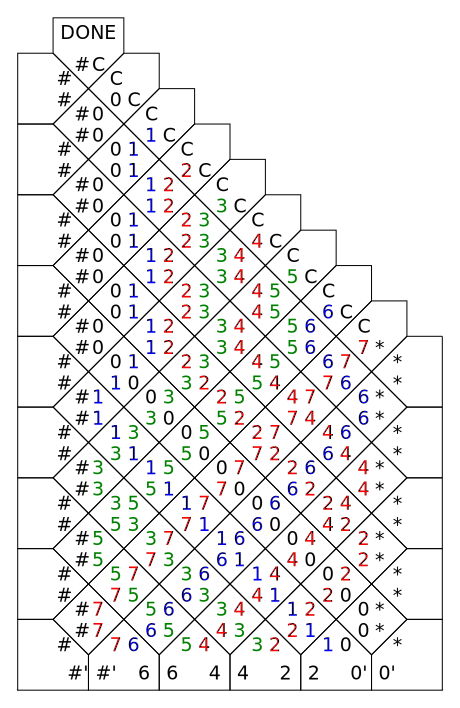
\includegraphics[scale=0.75]{./figures/3-color/3-color.pdf}
	\caption{3-color computation.}
	\label{fig:3-color}
\end{center}
\end{figure}
